\documentclass[14pt]{extarticle}
\usepackage{fontspec}
\usepackage{polyglossia}
\usepackage{amsmath}
\usepackage{amsfonts}
\usepackage{amssymb}
\usepackage{pgfplots}
\pgfplotsset{compat=1.18}

% Hebrew setup
\setdefaultlanguage{hebrew}
\setotherlanguage{english}
\newfontfamily\hebrewfont[Script=Hebrew]{Arial}

% Math font setup for proper Greek symbols
\usepackage{unicode-math}
\setmathfont{Latin Modern Math}

% Increase line spacing throughout document
\linespread{1.3}

\usepackage[margin=1in]{geometry}

% Left-aligned equation environment
\newenvironment{lefteqs}{%
    \begin{english}%
    \begin{flushleft}%
    \renewcommand{\arraystretch}{1.3}%
    $\begin{array}{@{}l@{}}%
}{%
    \end{array}$%
    \end{flushleft}%
    \end{english}%
}

\begin{document}

\begin{center}
    {\LARGE \textbf{מטלה 1 - פיסיקה של החלקיקים היסודיים    }}\\[0.5em]
    {\large שי רואימי - 318986270}\\[0.3em]
\end{center}

\hrule
\vspace{2em}

\textbf{\large שאלה 1}

\textbf{א)}
כפי שמתואר בשאלה, מדובר בדעיכה שקוראת באינטרקציה חזקה ולכן מסתכל על שימור מטען, ושימור מוזרות.
אציין שנדרש גם כי אנרגיית התוצרים תהיה נמוכה מאנרגיית החלקיק המקורי,
אבל ההתייחסות לזה היא בסעיף ב' אז אתעלם מזה בסעיף הזה.

$\Delta^-$ מורכב מ-$dds$, כלומר בעל מוזרות $0$ ומטען $-1$.

המזונים (mesons): $\pi^0 \, , \pi^+ \, , \pi^- \, \eta $ בעלי $S=0$ (אסמן מוזרות ב-$S$).

הבריונים (baryons): $n \, , p$ בעלי $S=0$. על מנת לספק את תנאי המטען רק הזוג $n + \pi^-$ מתאים.

המזונים בעלי $S\neq 0$ מקיימים $S=\pm 1$, כלומר יכולים להתאים עם ברויונים בעלי $S=\mp 1$.
לא קיימים בריונים באוקטט בעלי $S=1$ ולכן נסתכל רק על מזונים בעלי $S=1$ ובריונים בעלי $S=-1$.
רק הזוג $K^0 + \Sigma^-$ מתאים.

לסיכום הדעיכות של חלקיק זה הן:
\begin{lefteqs}
    \Delta^- \to n + \pi^- \\
    \Delta^- \to \Sigma^- + K^0
\end{lefteqs}

נעשה תהליך דומה עבור $\Sigma^{*+}$.
חלקיק זה מורכב מהקווארקים $uus$, כלומר בעל מוזרות $-1$ ומטען $+1$.

ל $n\, , p$ יש מוזרות $S=0$, והמזונים בעלי מוזרות $S=-1$ הם $\bar{K}^0 \, , K^-$.

הזוג $\bar{K}^0 + p$ מקיים את תנאי המוזרות והמטען.

בנוסף אליו, ייתכנו הזוגות:
\begin{lefteqs}
    \Sigma^{*+} \to \bar{K}^0 + p \\
    \Sigma^{*+} \to \Lambda + \pi^+ \\
    \Sigma^{*+} \to \Sigma^0 + \pi^+ \\
    \Sigma^{*+} \to \Sigma^+ + \pi^0 \\
    \Sigma^{*+} \to \Sigma^+ + \eta \\
    \Sigma^{*+} \to \Xi^0 + K^+ \\
\end{lefteqs}

נבדוק כעת את הדעיגה של $\Xi^{*-}$, נעבוד בצורה מסודרת יותר.
נעבור על רשימת הבריונים ונבדוק עבור על אחד אם ישנם זוגות מזונים שיכולים להתאים לדעיכה.

ראשית, $\Xi^{*-}$ מורכב מהקווארקים $dss$, בעל מטען $-1$ ומוזרות $-2$..

$n\, , p$ בעלי מוזרות 0, ולא קיימים מזרונים בעלי מוזרות $S=-2$ ולכן לא ייתכנו בדעיכה.

$\Lambda$ ו $\Sigma^0$ בעלי מוזרות $S=-1$ ומטען $0$ ולכן יתאים להם מזונים בעלי מוזרות $S=-1$ ומטען $-1$, כלומר הזוגות $(\Sigma^0 \, , K^-)  \, , (\Lambda \, , K^-)$

$\Sigma^+$ בעל מטען $=1$ ולא קיימים מזונים בעלי מטען $-2$ ולכן לא ייתכן.

$\Sigma^-$ בעל מטעו $-1$ ומוזרות $S=-1$, לכם יתאימו לו מזונים בעלי מטען $0$ ומוזרות $S=-1$, כלומר הזוג $(\Sigma^- \, , \bar{K}^0)$.

$\Xi^0$ בעל מטען $0$ ומוזרות $S=-2$, לכן יתאים לו מזון בעל מטען $-1$ ומוזרות $S=0$, כלומר הזוג $(\Xi^0 \, , \pi^-)$.

$\Xi^-$ בעל מטען $-1$ ומוזרות $S=-2$, לכן יתאים לו מזון בעל מטען $0$ ומוזרות $S=0$, כלומר הזוגות $(\Xi^- \, , \pi^0) \, , (\Xi^- \, , \eta)$

כלומר הדעיכות האפשריות של $\Xi^{*-}$ הן:
\begin{lefteqs}
    \Xi^{*-} \to \Sigma^0 + K^- \\
    \Xi^{*-} \to \Lambda + K^- \\
    \Xi^{*-} \to \Sigma^- + \bar{K}^0 \\
    \Xi^{*-} \to \Xi^0 + \pi^- \\
    \Xi^{*-} \to \Xi^- + \pi^0 \\
    \Xi^{*-} \to \Xi^- + \eta
\end{lefteqs}

\textbf{ב)}
נבדוק את דרישת המסה לכל אחת מהדעיכות בסעיף א'.

\begin{lefteqs}
    \Delta^- \to n + \pi^- \iff 1232 > 940 + 140 = 1080 \Rightarrow \text{possible} \\
    \Delta^- \to \Sigma^- + K^0 \iff 1232 \ngtr 1197 + 498 = 1695 \Rightarrow \text{not possible} \\

    \Sigma^{*+} \to \bar{K}^0 + p \iff 1385 \ngtr 498 + 938 = 1436 \Rightarrow \text{not possible} \\
    \Sigma^{*+} \to \Lambda + \pi^+ \iff 1385 > 1116 + 140 = 1256 \Rightarrow \text{possible} \\
    \Sigma^{*+} \to \Sigma^0 + \pi^+ \iff 1385 > 1193 + 140 = 1333 \Rightarrow \text{possible} \\
    \Sigma^{*+} \to \Sigma^+ + \pi^0 \iff 1385 > 1189 + 135 = 1324 \Rightarrow \text{possible} \\
    \Sigma^{*+} \to \Sigma^+ + \eta \iff 1385 \ngtr 1189 + 549 = 1738 \Rightarrow \text{not possible} \\
    \Sigma^{*+} \to \Xi^0 + K^+ \iff 1385 \ngtr 1315 + 494 = 1809 \Rightarrow \text{not possible} \\

    \Xi^{*-} \to \Sigma^0 + K^- \iff 1533 \ngtr 1193 + 494 = 1687 \Rightarrow \text{not possible} \\
    \Xi^{*-} \to \Lambda + K^- \iff 1533 \ngtr 1116 + 494 = 1610 \Rightarrow \text{not possible} \\
    \Xi^{*-} \to \Sigma^- + \bar{K}^0 \iff 1533 \ngtr 1197 + 498 = 1695 \Rightarrow \text{not possible} \\
    \Xi^{*-} \to \Xi^0 + \pi^- \iff 1533 > 1315 + 140 = 1455 \Rightarrow \text{possible} \\
    \Xi^{*-} \to \Xi^- + \pi^0 \iff 1533 > 1321 + 135 = 1456 \Rightarrow \text{possible} \\
    \Xi^{*-} \to \Xi^- + \eta \iff 1533 \ngtr 1321 + 549 = 1870 \Rightarrow \text{not possible}
\end{lefteqs}

\vspace{3em}
\hrule
\vspace{2em}

\textbf{\large שאלה 2}
עם קווארק בטעם אחד, קיימת קומבינציה אחת אפשרית (לדוגמא עבור $u$ קיים רק $uuu$)

עם 2 טעמים שונים ניתן להרכיב 4 בריונים: $u + d \Rightarrow (uud, udd, uuu, ddd)$

עם 3 טעמים שונים ניתן להרכיב 10: $(uuu, ddd, sss, uud, udd, uus, uss, dss, dds, uds)$

נפרק את החישוב לסוגי קומבינציות. עבור $n$ קווארקים יש $n$ יש $n$ קומבינציות בהן כולם מאותו סוג.
לדוגמא, עבור $n=1$ יש רק $uuu$ ועבור $n=3$ יש $uuu, ddd, sss$.

שנית, עבור $n$ קווארקים יש $n(n-1)$ קומבינציות בהן 2 קווארקים דומים ואחד שונה.
לדוגמא, עבור $n=3$ יש $3 \cdot 2 = 6$ קומבינציות: $(uud, udd, uus, uss, dss, dds)$.

לבסוף, עבור $n$ קווארקים יש $\binom{n}{3}$ קומבינציות בהן כל הקווארקים שונים.
לדוגמא, עבור $n=3$ יש $\binom{3}{3} = 1$ קומבינציה: $(uds)$.

לכן סך הקומבניציות הוא:

\begin{lefteqs}
    n + n(n-1) + \binom{n}{3} = n + n^2 - n + \frac{n(n-1)(n-2)}{6} = n^2 + \frac{n(n-1)(n-2)}{6} \\
    = \frac{n}{6} \left( 6n + (n-1)(n-2) \right) = \frac{n}{6} \left( 6n + n^2 - 3n + 2 \right) \\
    = \frac{n}{6} \left( n^2 + 3n + 2 \right) = \frac{n(n+1)(n+2)}{6}
\end{lefteqs}

כלומר הנוסחא היא:
\begin{lefteqs}
    \text{Quark Combinations} = \frac{n(n+1)(n+2)}{6}
\end{lefteqs}

נציב את הערכים $n=1,2,3,4,5,6$:
\begin{lefteqs}
    \frac{1 \cdot 2 \cdot 3}{6} = 1 \\
    \frac{2 \cdot 3 \cdot 4}{6} = 4 \\
    \frac{3 \cdot 4 \cdot 5}{6} = 10 \\
    \frac{4 \cdot 5 \cdot 6}{6} = 20 \\
    \frac{5 \cdot 6 \cdot 7}{6} = 35 \\
    \frac{6 \cdot 7 \cdot 8}{6} = 56
\end{lefteqs}

\vspace{3em}
\hrule
\vspace{2em}

\textbf{\large שאלה 3}
הדיאגרמה תראה כך:
\begin{center}
    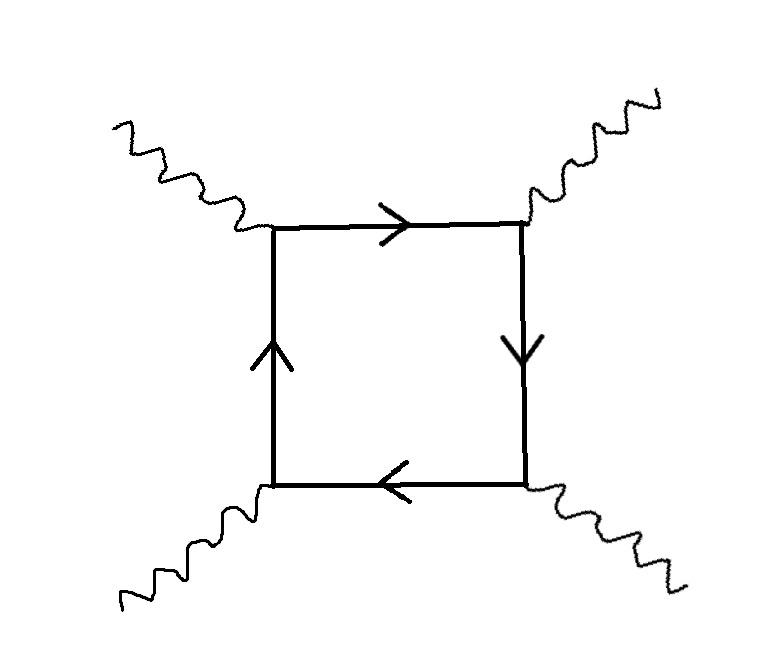
\includegraphics[width=0.5\textwidth]{maman_1_q3.png}
\end{center}

באלקטרונידמיקה קוונטית (QED) ישנו רק קודוקד בסיסי אחד (איני בטוח בתרגום הישיר של vertex בקונטקסט הזה)
שהוא אלקטרון שפולט או בולע פוטון.

לכן בדיאגרמת פיינמן אין אינטרקציה ישירה בין פוטונים אלא רק דרך אלקטרונים.

על מנת להרכיב את הדיאגרמה של פיזור דלבריק, כל אחד מארבעת הפוטונים החיצוניים (שניים נכנסים ושניים יוצאים)
חייב להתחבר לקודקוד משלו, ולכן נדרשים ארבעה קודקודים.
בכל קודקוד קו האלקטרון נכנס ויוצא, וקו האלקטרון היוצא מקודקוד אחד נכנס לקודקוד הבא.

\vspace{3em}
\hrule
\vspace{2em}

\textbf{\large שאלה 5}

ראשית נצייר את שתי הדיגרמות פיינמן עבור הדעיכות.

הדעיכה $\Xi^{-} \to \Lambda + \pi^{-}$:

\begin{center}
    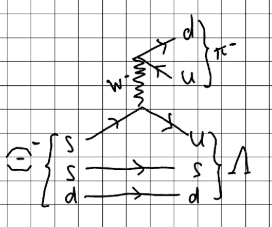
\includegraphics[width=0.5\textwidth]{maman_1_q5_d1.png}
\end{center}

הדעיכה $\Xi^{-} \to n + \pi^{-}$:

\begin{center}
    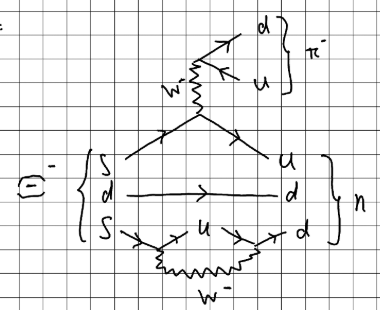
\includegraphics[width=0.5\textwidth]{maman_1_q5_d2.png}
\end{center}

הדעיכה $\Xi^{-} \to n + \pi^{-}$ דורשת שני אקסטרה $W^-$ ביחס לדעיכה הראשונה, ולכן תהיה תקרה בסיכוי נמוך יותר.

כלומר, ההתפרקות ל $\Lambda + \pi^-$ סבירה יותר.

\newpage
\textbf{\large שאלה 6}

\textbf{א)}
\begin{lefteqs}
    m(\Sigma^0) = 1193 \frac{MeV}{c^2} \\
    m(\Lambda) = 1116 \frac{MeV}{c^2} \\
    m(\pi^0) = 135 \frac{MeV}{c^2} \\
\end{lefteqs}

סכום המסות של התוצרים ($1116 + 135 = 1251 \frac{MeV}{c^2}$) גדול ממסת החלקיק המקורי.
כלומר התהליך אינו אפשרי בגלל שהוא מפר את חוק שימור האנרגיה.

\textbf{ב)}
התהליך לא אפשרי כי לא מתקיים שימור מספר בריוני.
באגף אחד יש פרוטון בעל מספר בריון 1 ובאגף השני אין בריונים.

\textbf{ג)}
מתקיים שימור מטען, אנרגיה, ומספר בריוני, ומספר לפטוני, ולכן התהליך אפשרי.
נשים לב כי יש שינוי טעם ($s \to d$).
באינטרקציה חזקה ואלקטרומנטית מתקיים שימור טעם ולכן אינטרקציות אלו לא מתאפשרות בתהליך הזה.
כלומר, האינטרקציה היא חלשה.

\textbf{ד)}
לא אפשרית, כי לא מתקיים שימור מספר בריוני.

\textbf{ה)}
לא אפשרית, כי לא מתקיים שימור מטען חשמלי.

\textbf{ו)}
מתקיים שימור מספר בריוני, מספר לפטוני, מטען ואנרגיה, ולכן התהליך אפשרי.
מתקיים שימור טעם, באגף שמאל $n + \bar{n} \, (udd + \bar{u} \bar{d} \bar{d})$,
ובאגף ימין $\pi^+ + \pi^- + \pi^0 \, (u\bar{d} + d\bar{u} + 0)$.
בשני האגפים הטעם נטו של כל קווארק הוא 0.

מאשר שהטעם נשמר ומשתתפים בתהליך רק הדרונים, האינטרקציה החזקה יכולה לגרום לו.
כאשר האינטרקציה החזקה אפשרית, היא הדומיננטית ולכן האינטרקציה היא חזקה.

\textbf{ז)}
מתקיים שימור אנרגיה, מטען ומספר לפטוני (אלטקרון וניטרינו) ומספר בריוני ולכן התהליך אפשרי.
נשים לב כי מתקיים שינוי טעם ($s \to u$), ולכן האינטרקציה היא חלשה.
בנוסף, בתוצר הסופי מופיע ניטרינו ורק אינטרקציות חלשות יכולות לייצר ניטרינו, ולכן האינטרקציה היא חלשה.

\textbf{ח)}
לא מתקיים שימור מספר לפטוני ולכן התהליך לא אפשרי.
באגף שמאל אין לפטונים והמספר הלפטוני הוא 0,
ובאגף ימין יש אלקטרון וניטרינו, ולכן המספר הלפטוני הוא 2.

\textbf{ט)}
מתקיים שימור מטען (המטען של אנטי-פרוטון הוא -1),
שימור אנרגיה, שימוש מספר בריוני ומספר לפטוני, ולכן התהליך אפשרי.

מכיוון שהטעם נשמר ומשתתפים בתהליך רק הדרונים, האינטרקציה החזקה יכולה לגרום לו.
כאשר האינטרקציה החזקה אפשרית, היא הדומיננטית ולכן האינטרקציה היא חזקה.

\textbf{י)}
לא אפשרית כי לא מתקיים שימור מספר לפטוני.
נשים לב כי מתקיים שימור מספר אלקטרון (אלקטרון ואנטי ניוטרינו-אלקטרון), אך לא מתקיים שימור מספר $\mu$.

\newpage
\textbf{\large שאלה 7}
\textbf{א)}
\begin{center}
    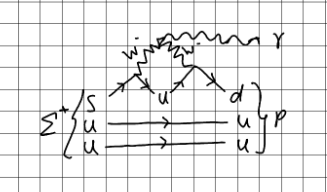
\includegraphics[width=0.5\textwidth]{maman_1_q7_d1.png}
\end{center}
הכוחות המעורבים הם אלקטרומנטיים והכוח החלש.

\textbf{ב)}
\begin{center}
    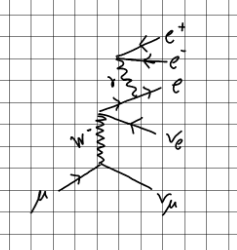
\includegraphics[width=0.5\textwidth]{maman_1_q7_d2.png}
\end{center}
הכוחות המעורבים הם אלקטרומנטיים והכוח החלש.



\end{document}